\subsection{VAE}
\subsubsection{Introduction to VAE}
The \textbf{Variational Auto-encoder} (VAE) \cite{kingma2014} is an artificial neural network whose encoder and decoder are connected through a probabilistic latent space, corresponding to the parameters of a variational distribution.
\begin{figure}[H]
    \centering
    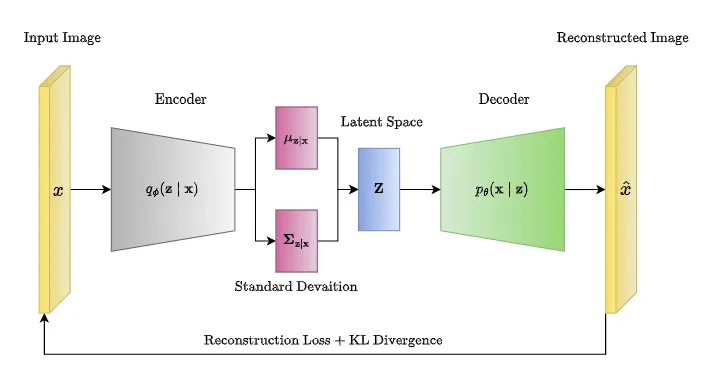
\includegraphics[width=1\linewidth]{assets/vae_structure.png}
    \caption{Structure of a Variational Auto-encoder, picture from \cite{shende2023}}
    \label{fig:vae structure}
\end{figure}
The encoder receives as input a tensor representing an image extracted from a dataset, and it maps it into a distribution within the latent space, parametrized by a mean vector $\mu$ and a log-variance vector $\log\sigma^2$. The network predicts the logarithm of the variance instead of the standard deviation, so that its output is unconstrained in sign while $\sigma$ remains positive.
\\\\
The decoder, instead, maps from the latent space back to the input space.
\\\\
The VAE's parameters are optimized via gradient descent, however the sampling of the latent variable $z$ introduces stochasticity, making the gradient of the loss with respect to the model parameters non-differentiable. A technique known as \textbf{Reparameterization Trick} is employed to address this problem, which expresses the sampling operation in a way that separates the deterministic and stochastic parts, enabling gradient flow through the deterministic part. So instead of directly sampling $z$ as $z\sim N(\mu,\sigma^2)$, which is non-differentiable with respect to $\mu$ and $\sigma$, it sample an auxiliary variable $\epsilon$ from a standard normal distribution $N(0,I)$, and then it expresses $z$ as $z=\mu+\sigma\cdot\epsilon$, which is now a differentiable function of $\mu$ and $\sigma$.
\\
\subsubsection{Components of VAE}
The two primary components of the VAE are:
\paragraph{Encoder}
\hfill \break
The encoder’s architecture consists of four 2D convolution layers, one flatten layer and one dense layer. The input received by this module, which is a 1-channel $28\times28$ image, passes through the convolutional layers -- using 32, 64, 64 and 64 filters respectively -- to extract features, then the feature maps is flattened and its dimensionality is reduced using a dense layer; finally the encoder outputs the mean and the log-variance of the latent space distribution and samples the latent vector $z$.
\begin{figure}[H]
    \centering
    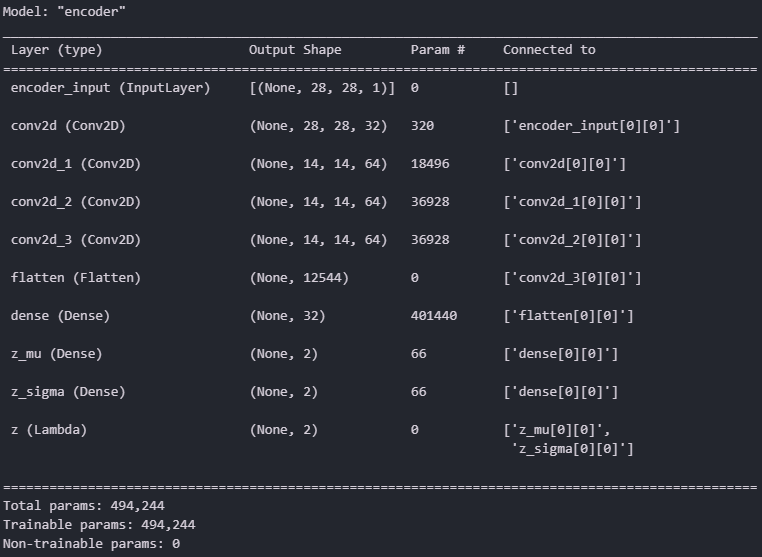
\includegraphics[width=1\linewidth]{assets/encoder_vae.png}
    \caption{Structure of a VAE Encoder}
    \label{fig:vae encoder}
\end{figure}
\paragraph{Decoder}
\hfill \break
The decoder’s architecture consists of a dense layer, a reshape layer and two 2D transposed convolution layers. The input of the module is the latent vector that, through the dense and reshape layers, it is transformed back into a tensor, matching the shape of the last convolution layer of the encoder; finally the convolution layers generate the reconstructed image with the same number of channels as the original input image.
\begin{figure}[H]
    \centering
    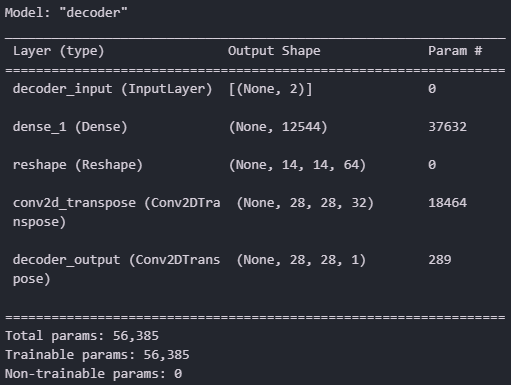
\includegraphics[width=1\linewidth]{assets/decoder_vae.png}
    \caption{Structure of VAE Decoder}
    \label{fig:vae decoder}
\end{figure}
\subsubsection{Training Process}
The optimization of VAE is achieved through the maximization of the \textbf{Evidence Lower Bound} (ELBO), consisting of two terms: the \textbf{Reconstruction Loss} and the \textbf{Regularization Term} (Kullback–Leibler Divergence).\\Given the input data $x$, the latent variable $z$, the encoder network $q_\phi(z\vert x)$, the decoder network $p_\theta(x\vert z)$, the prior distribution over the latent variables $p(z)$, the reconstruction loss $\mathbb{E}_{q_{\phi}(z\vert x)}[log\ p_\theta(x\vert z)]$, and the KL divergence $KL(q_\phi(z\vert x)\ \vert\vert\ p(z))$, the loss is computed as:
\\
\begin{equation}
L(\theta,\phi;x)=\mathbb{E}_{q_{\phi}(z\vert x)}[log\ p_\theta(x\vert z)]-KL(q_\phi(z\vert x)\ \vert\vert\ p(z))
\end{equation}
The VAE is trained with a custom loop, consisting of three main steps: \textbf{forward pass}, \textbf{loss calculation} and \textbf{backward pass}. During the forward pass, the input data is passed through the encoder to get the mean and log variance of the latent distribution, then the latent vector z is sampled using the reparamentrization trick, and finally z is passed through the decoder to get the reconstructed data. The loss calculation step computes the reconstruction loss between the input data and the reconstructed data, the KL divergence, and then sums them up to compute the total loss. Finally, in the backward pass the total loss is backpropagated to update the parameters of the encoder and decoder.
\\\\
The model is trained for up to 100 epochs using a batch size of 100 and an Adam optimizer \cite{kingma2015adam} with learning rate of 0.001, with early stopping monitoring the loss.
\\\\
To test the goodness of the model in the context of compress sensing, two versions of the VAE have been generated: one with the dimension of the latent vector equal to 20, and the other equal to 30. After using both of them, it’s possible to conclude that they lead to good results, as shown in the Results section.
\subsection{Model results}
The following graph shows the output mean vector produced by the encoder with the test set provided by the MNIST dataset. For the sake of simplicity, this result is obtained with a latent dimension equal to 2.
\begin{figure}[H]
    \centering
    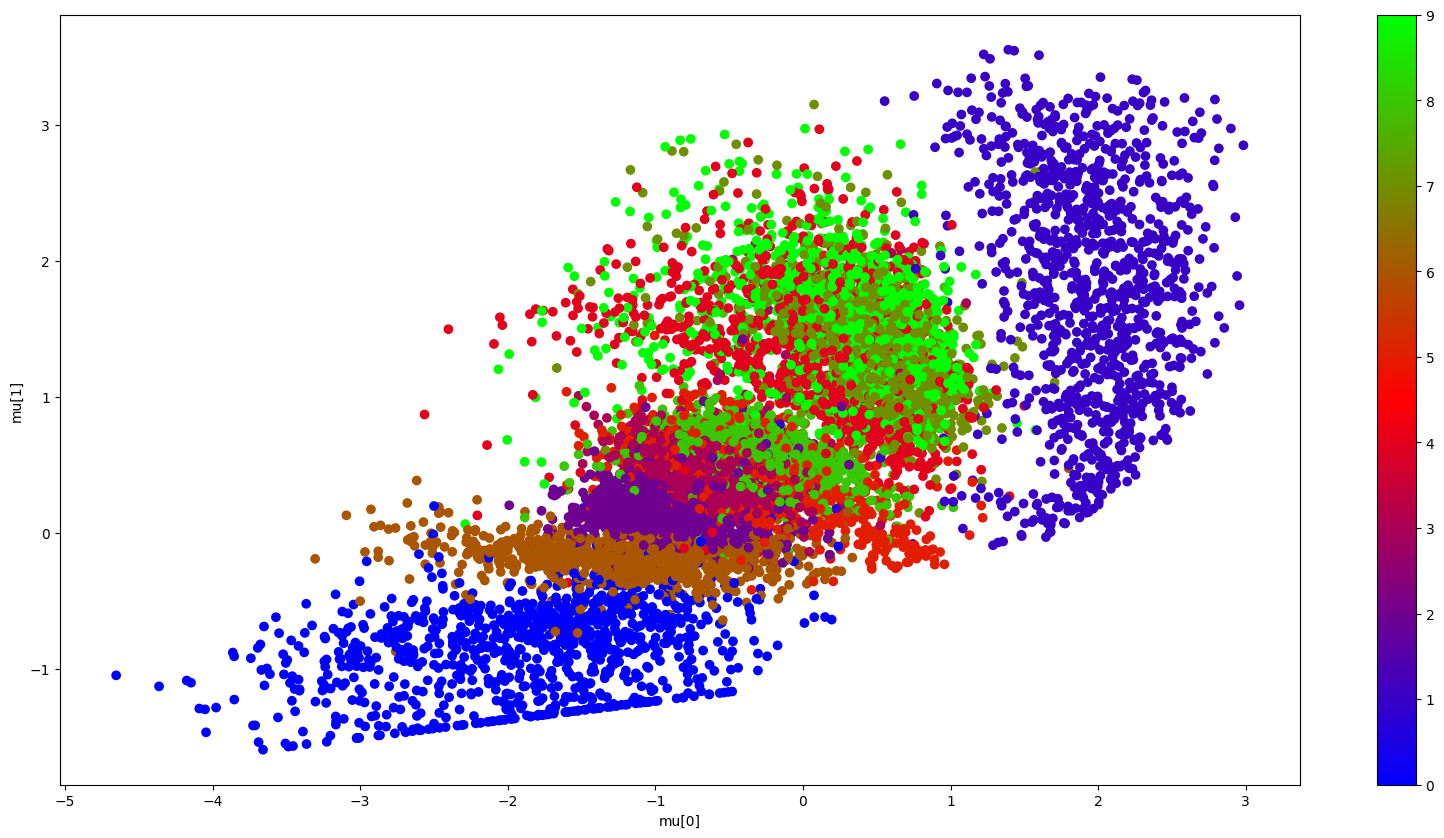
\includegraphics[width=0.89\linewidth]{assets/output_encoder.png}
    \caption{Plotted output of the encoder, each color represents a specific digit}
    \label{fig:vae latent space}
\end{figure}
\hfill \break
By observing the data in the graph, we can predict the behaviour of the decoder. Infact, if we assume it receives as input the vector $[-2,-1]$, we expect the output to depict with good precision the number 0, as represented by the blue color in the lateral colorbar. The image reconstruction is shown in the image below.
\begin{figure}[H]
    \centering
    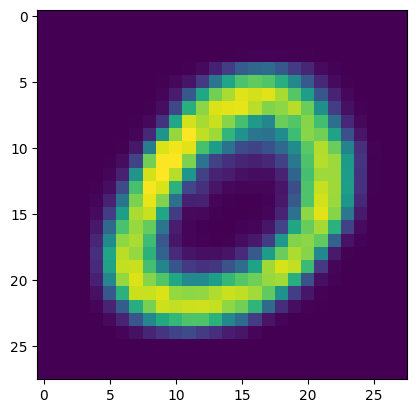
\includegraphics[width=0.5\linewidth]{assets/output_decoder.png}
    \caption{Output of the decoder for the input vector $[-2,-1]$}
    \label{fig:vae decoder output}
\end{figure}